\documentclass[11pt]{article}
\usepackage[utf8]{inputenc}
\usepackage[T1]{fontenc}
\usepackage{amsmath, amssymb, mathtools}
\usepackage[margin=1in]{geometry}
\usepackage{xcolor}
\usepackage{listings}
\usepackage{hyperref}
\usepackage{enumitem}
\usepackage{graphicx}
\usepackage{fourier-orns}
\usepackage{pgfornament}
\usepackage{booktabs}
\usepackage{array}
\usepackage{epigraph}
\setlength{\epigraphwidth}{0.55\textwidth}
\renewcommand{\epigraphflush}{center}
\renewcommand{\epigraphrule}{0pt}

\lstset{
  language=Python,
  basicstyle=\ttfamily\small,
  keywordstyle=\color{blue!70!black},
  commentstyle=\color{gray!70},
  stringstyle=\color{green!40!black},
  showstringspaces=false,
  frame=single,
  breaklines=true,
  columns=fullflexible
}

\hypersetup{colorlinks=true, linkcolor=blue!60!black, urlcolor=blue!60!black}

% ----------------------------------------------------------------
\begin{document}
% ----------------------------------------------------------------

\begin{center}
  {\large\scshape University of Austin}\\[0.5cm]
  {\Large\bfseries Linear Algebra: Mathematics and Computation}\\[0.4cm]
  \hrulefill\hspace{0.25cm}{\large\leafleft\aldine\leafright}\hspace{0.25cm}\hrulefill\\[0.4cm]
  {\large Lecture~1 $\cdot$ A First Look: Signals on an Infinite Grid}\\[0.2cm]
  {\normalsize Spring 2026}
\end{center}

\epigraph{\itshape Come play my game}{``Breathe'' --- \textsc{The Prodigy} (1994)}

\bigskip\noindent
\textit{This note introduces the course's central question through an
example you will not fully understand today.  That is intentional.
Everything here will be completely transparent by the end of the course.
For now: run the code, look at the pictures, notice what is strange.}

% ================================================================
\section*{Motivation: Conway's Game of Life}
% ================================================================

In 1970 John Conway published a remarkably simple rule for a
\emph{cellular automaton} on the infinite square lattice
$\mathbb{Z}^2$.  Each cell is either \emph{alive} or \emph{dead}.
At each tick:
\begin{itemize}[nosep]
  \item an alive cell \emph{survives} iff it has 2 or 3 alive neighbours
        (of its 8 Moore neighbours);
  \item a dead cell \emph{is born} iff it has exactly 3 alive neighbours.
\end{itemize}
From this rule emerges extraordinary complexity: stable structures,
periodic \emph{oscillators}, and --- most remarkably --- \emph{gliders}:
five-cell patterns that translate themselves diagonally one step every
four ticks.

\begin{lstlisting}
import numpy as np
import matplotlib.pyplot as plt
import matplotlib.animation as animation

def gol_step(grid):
    """One step of Conway's Game of Life (toroidal boundary conditions)."""
    N = np.zeros_like(grid)
    for di in (-1, 0, 1):
        for dj in (-1, 0, 1):
            if di == 0 and dj == 0:
                continue
            N += np.roll(np.roll(grid, di, axis=0), dj, axis=1)
    return ((grid == 1) & ((N == 2) | (N == 3))) | ((grid == 0) & (N == 3))

# Standard glider (top-left corner of a 32x32 grid)
G = np.zeros((32, 32), dtype=int)
glider = [(1,0),(2,1),(0,2),(1,2),(2,2)]
for r, c in glider:
    G[r, c] = 1

fig, axes = plt.subplots(1, 5, figsize=(14, 3))
for ax, t in zip(axes, range(0, 20, 4)):
    ax.imshow(G, cmap='binary', interpolation='nearest')
    ax.set_title(f't = {t}'); ax.axis('off')
    for _ in range(4): G = gol_step(G)
plt.suptitle("GoL glider: moves one step diagonally every 4 ticks", y=1.02)
plt.tight_layout()
plt.savefig("fig_glider.png"); plt.show()
\end{lstlisting}

\begin{figure}[h!]
  \centering
  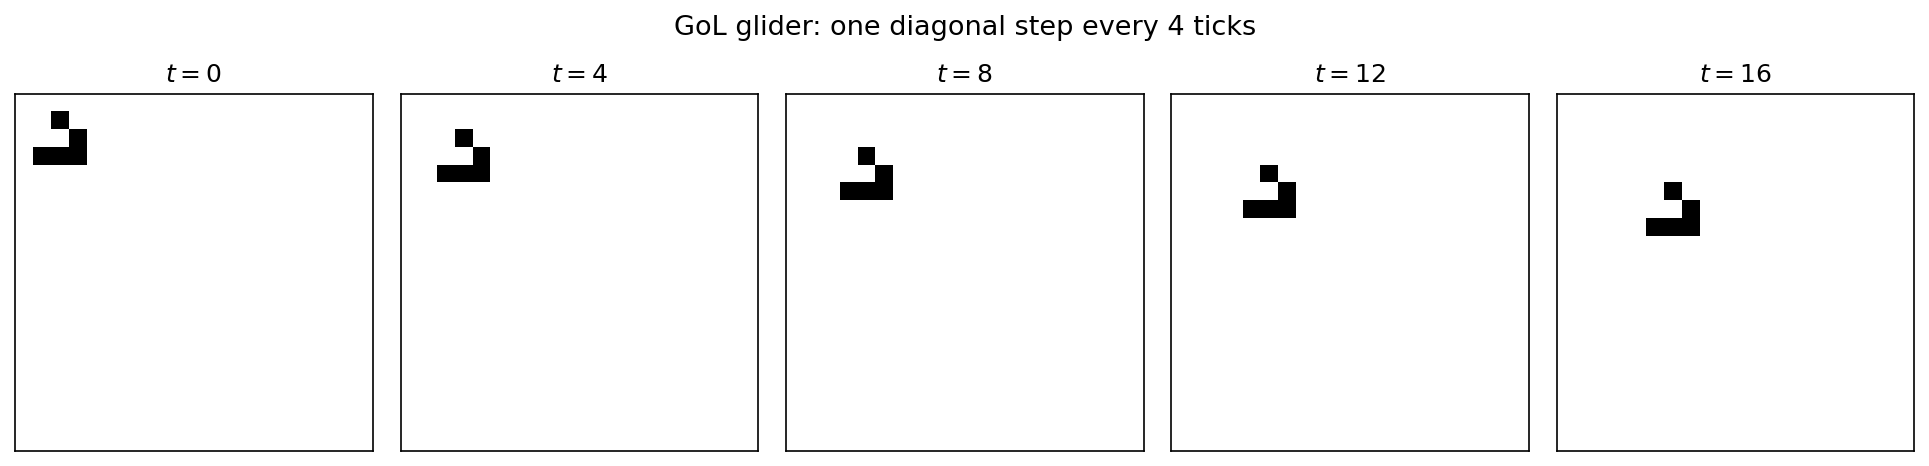
\includegraphics[width=\textwidth]{fig_glider.png}
  \caption{The standard GoL glider over 20 ticks (every 4th frame shown).
    The pattern shifts exactly one cell diagonally every 4 steps ---
    a periodic translation along the main-diagonal axis.}
\end{figure}

\noindent
The glider moves diagonally.  Is that a coincidence, or is there
something about the lattice that \emph{forces} long-lived structures
to move diagonally?  This is the question we will partially answer today
--- and fully answer by the end of the course.


% ================================================================
\section*{The Linear Version}
% ================================================================

Conway's rule is \emph{non-linear}: the ``exactly 3 neighbours'' condition
is a threshold function, not a linear combination of cell values.
Non-linear maps are hard.

We replace it with a \textbf{linear transfer rule}.  Instead of binary
states, each cell carries a real number $u_{m,n}(t) \in \mathbb{R}$
(think of it as ``activity level'' or ``excitation'').  The rule uses
only the two diagonal neighbours in the north-east and south-west
directions:
\begin{equation}\label{eq:T}
  \boxed{
    u_{m,n}(t+1) \;=\; p\,u_{m+1,\,n+1}(t) \;+\; q\,u_{m-1,\,n-1}(t)
  }
\end{equation}
with parameters
\[
  p = 1.2, \qquad q = 0.8.
\]

\medskip\noindent
\textbf{Reading the rule.}
The activity at cell $(m,n)$ at time $t+1$ is a weighted sum of the
activity at the north-east neighbour $(m{+}1,n{+}1)$ (weight $1.2$:
amplified, like an enemy signal arriving from the north-east) and the
south-west neighbour $(m{-}1,n{-}1)$ (weight $0.8$: attenuated, like
a player signal coming from the south-west).  The rule couples only
the \emph{main diagonal} axis $\{(m{+}k,n{+}k) : k\in\mathbb{Z}\}$
through each cell.

\medskip\noindent
We write $T$ for the \emph{transfer operator} defined by
\eqref{eq:T}, acting on functions $\mathbb{Z}^2\to\mathbb{R}$.
After $t$ steps the field is $T^t u_0$.

\medskip\noindent
\textbf{Questions.}
\begin{itemize}[nosep]
  \item If you place a localised ``blip'' at the origin, does it grow
    or decay?  In what direction does it spread?
  \item Are there initial conditions that grow, and others that decay?
  \item Is the answer different along the two diagonal axes of the grid
    --- the main diagonal $(+1,+1)$ and the anti-diagonal $(+1,-1)$?
\end{itemize}


% ================================================================
\section*{Python: Exploring on a Large Finite Grid}
% ================================================================

\noindent
We approximate $\mathbb{Z}^2$ by an $N\times N$ grid with
\emph{periodic} (toroidal) boundary conditions.

\begin{lstlisting}
import numpy as np
import matplotlib.pyplot as plt
from numpy.fft import fft2, ifft2, fftshift

N = 256   # grid size; approximates Z^2 for patterns much smaller than N

def step(u, p=1.2, q=0.8):
    """One step of the transfer rule: u[m,n] <- p*u[m+1,n+1] + q*u[m-1,n-1]."""
    # np.roll(u, -1, axis=0) shifts rows upward: u[m,n] <- u[m+1,n]
    return p * np.roll(np.roll(u, -1, axis=0), -1, axis=1) \
         + q * np.roll(np.roll(u, +1, axis=0), +1, axis=1)

def simulate(u0, T):
    u = u0.copy()
    frames = [u.copy()]
    for _ in range(T):
        u = step(u)
        frames.append(u.copy())
    return frames
\end{lstlisting}

\subsection*{Experiment 1: a localised blip}

\begin{lstlisting}
u0 = np.zeros((N, N))
u0[N//2, N//2] = 1.0            # single nonzero cell at centre

frames = simulate(u0, T=40)

fig, axes = plt.subplots(1, 4, figsize=(14, 4))
for ax, t in zip(axes, [0, 10, 20, 40]):
    im = ax.imshow(frames[t], cmap='seismic', vmin=-3, vmax=3,
                   origin='lower', extent=[-N//2, N//2, -N//2, N//2])
    ax.set_title(f't = {t}'); ax.set_xlabel('m'); ax.set_ylabel('n')
plt.suptitle("Evolution of a single-cell blip under rule (1)")
plt.tight_layout(); plt.savefig("fig_blip.png"); plt.show()
\end{lstlisting}

\begin{figure}[h!]
  \centering
  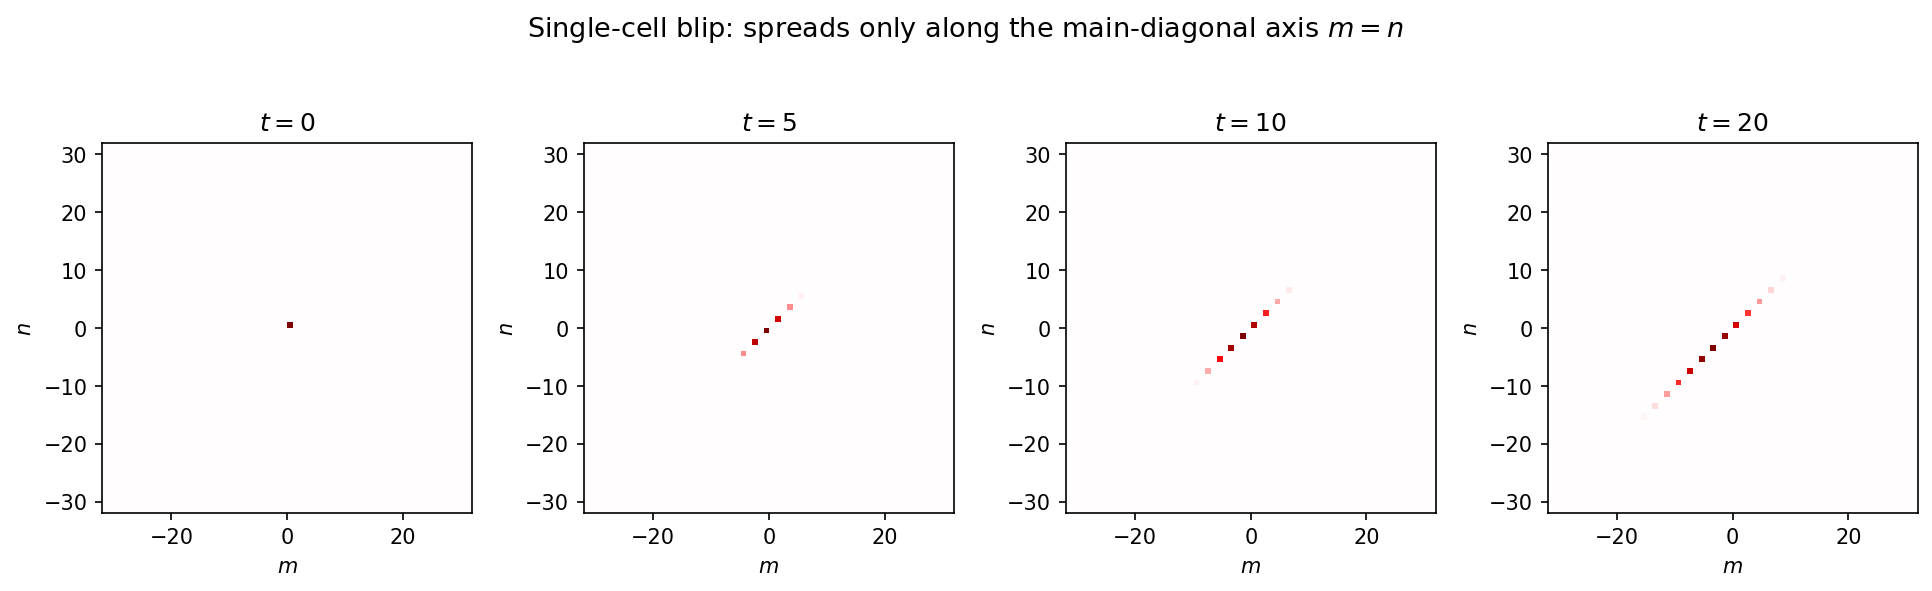
\includegraphics[width=\textwidth]{fig_blip.png}
  \caption{A single-cell blip at $t=0$ evolves under rule~\eqref{eq:T}.
    The nonzero region spreads exclusively along the main-diagonal axis $m=n$
    --- the direction the rule couples.}
\end{figure}

\noindent
Observe: the blip spreads \emph{only along the main diagonal axis}
$m = n$ --- exactly the axis the rule couples.  After $t$ steps the
nonzero cells form a segment of the main diagonal.  The \emph{other}
diagonal axis $m = -n$ (the anti-diagonal) carries no signal.

\medskip
\textbf{Total energy and peak value.}

\begin{lstlisting}
energies = [np.sum(np.abs(f)) for f in frames]
max_vals  = [np.max(np.abs(f))  for f in frames]
# By the binomial theorem, sum_d C(t,j)*p^j*q^{t-j} = (p+q)^t exactly.
print(f"L1 norm at t=20:  {energies[20]:.2e}  (predicted: {(p+q)**20:.2e})")
# The peak sits at j* = t*p/(p+q); local CLT gives (p+q)^t / sqrt(2*pi*t*p*q/(p+q)^2).
import numpy as np
def peak_theory(t):
    return (p+q)**t / np.sqrt(2*np.pi*t*p*q/(p+q)**2)
print(f"Peak at t=20:     {max_vals[20]:.2e}  (theory: {peak_theory(20):.2e})")
\end{lstlisting}

\begin{figure}[h!]
  \centering
  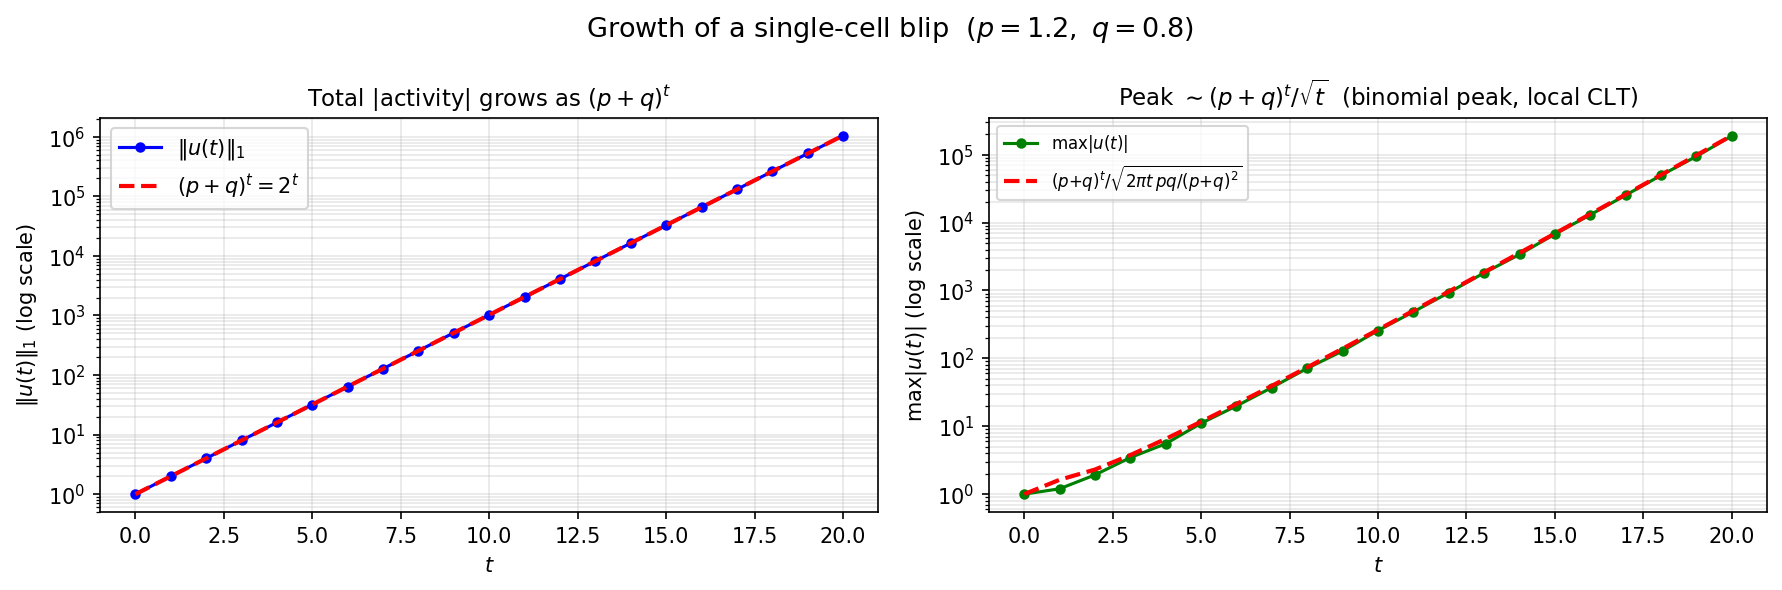
\includegraphics[width=\textwidth]{fig_blip_growth.png}
  \caption{%
    \textbf{Left:} total $L^1$ activity grows exactly as $(p+q)^t = 2^t$
    (binomial theorem: $\sum_j\binom{t}{j}p^j q^{t-j} = (p+q)^t$).
    \textbf{Right:} the peak cell value, achieved at diagonal offset
    $d^* \approx (p-q)t/(p+q) = 0.2t$ steps NE, grows as
    $(p+q)^t/\sqrt{t}$ --- the local CLT approximation to the binomial
    peak $\binom{t}{j^*}p^{j^*}q^{t-j^*}$ with $j^* = tp/(p+q)$.
    Dashed lines show the theoretical predictions; dots are simulation.}
\end{figure}

\noindent
The $L^1$ norm is \emph{exactly} $(p+q)^t = 2^t$ at every step --- no transient.
This follows from the binomial theorem: after $t$ steps the value at diagonal
position $d = 2j-t$ is $\binom{t}{j}p^j q^{t-j}$, and summing over all $j$
gives $(p+q)^t$.  The peak, however, grows only as $(p+q)^t/\sqrt{t}$:
the binomial distribution spreads over a segment of length $O(\sqrt{t})$,
diluting the peak by that factor.
Neither $p = 1.2$ nor $q = 0.8$ alone controls the $L^1$ growth --- it is
always their \emph{sum} $p + q = 2$.


\subsection*{Experiment 2: initialise along each diagonal}

Now we seed the grid with a \emph{striped} initial condition along
each of the two diagonal axes.

\begin{lstlisting}
m_idx, n_idx = np.meshgrid(np.arange(N), np.arange(N), indexing='ij')

def wave(k, direction='anti'):
    """
    direction='anti' : stripe along the anti-diagonal axis m - n = const
                       i.e.  u_{m,n} = exp(2*pi*i*k*(m-n)/N)
    direction='main' : stripe along the main diagonal axis m + n = const
                       i.e.  u_{m,n} = exp(2*pi*i*k*(m+n)/N)
    """
    if direction == 'anti':
        phase = 2 * np.pi * k * (m_idx - n_idx) / N
    else:
        phase = 2 * np.pi * k * (m_idx + n_idx) / N
    return np.cos(phase)      # take real part

K = 8   # 8 full oscillations across the grid

u_anti = wave(K, 'anti')
u_main = wave(K, 'main')

frames_anti = simulate(u_anti, T=20)
frames_main = simulate(u_main, T=20)

fig, axes = plt.subplots(2, 5, figsize=(16, 7))
for j, t in enumerate([0, 3, 7, 12, 20]):
    axes[0, j].imshow(frames_anti[t], cmap='seismic', vmin=-3, vmax=3,
                      origin='lower')
    axes[0, j].set_title(f'anti-diag, t={t}'); axes[0, j].axis('off')
    axes[1, j].imshow(frames_main[t], cmap='seismic', vmin=-3, vmax=3,
                      origin='lower')
    axes[1, j].set_title(f'main-diag, t={t}'); axes[1, j].axis('off')
plt.suptitle("Top: anti-diagonal stripe  |  Bottom: main-diagonal stripe "
             f"(K={K} full waves)")
plt.tight_layout(); plt.savefig("fig_stripes.png"); plt.show()
\end{lstlisting}

\begin{figure}[h!]
  \centering
  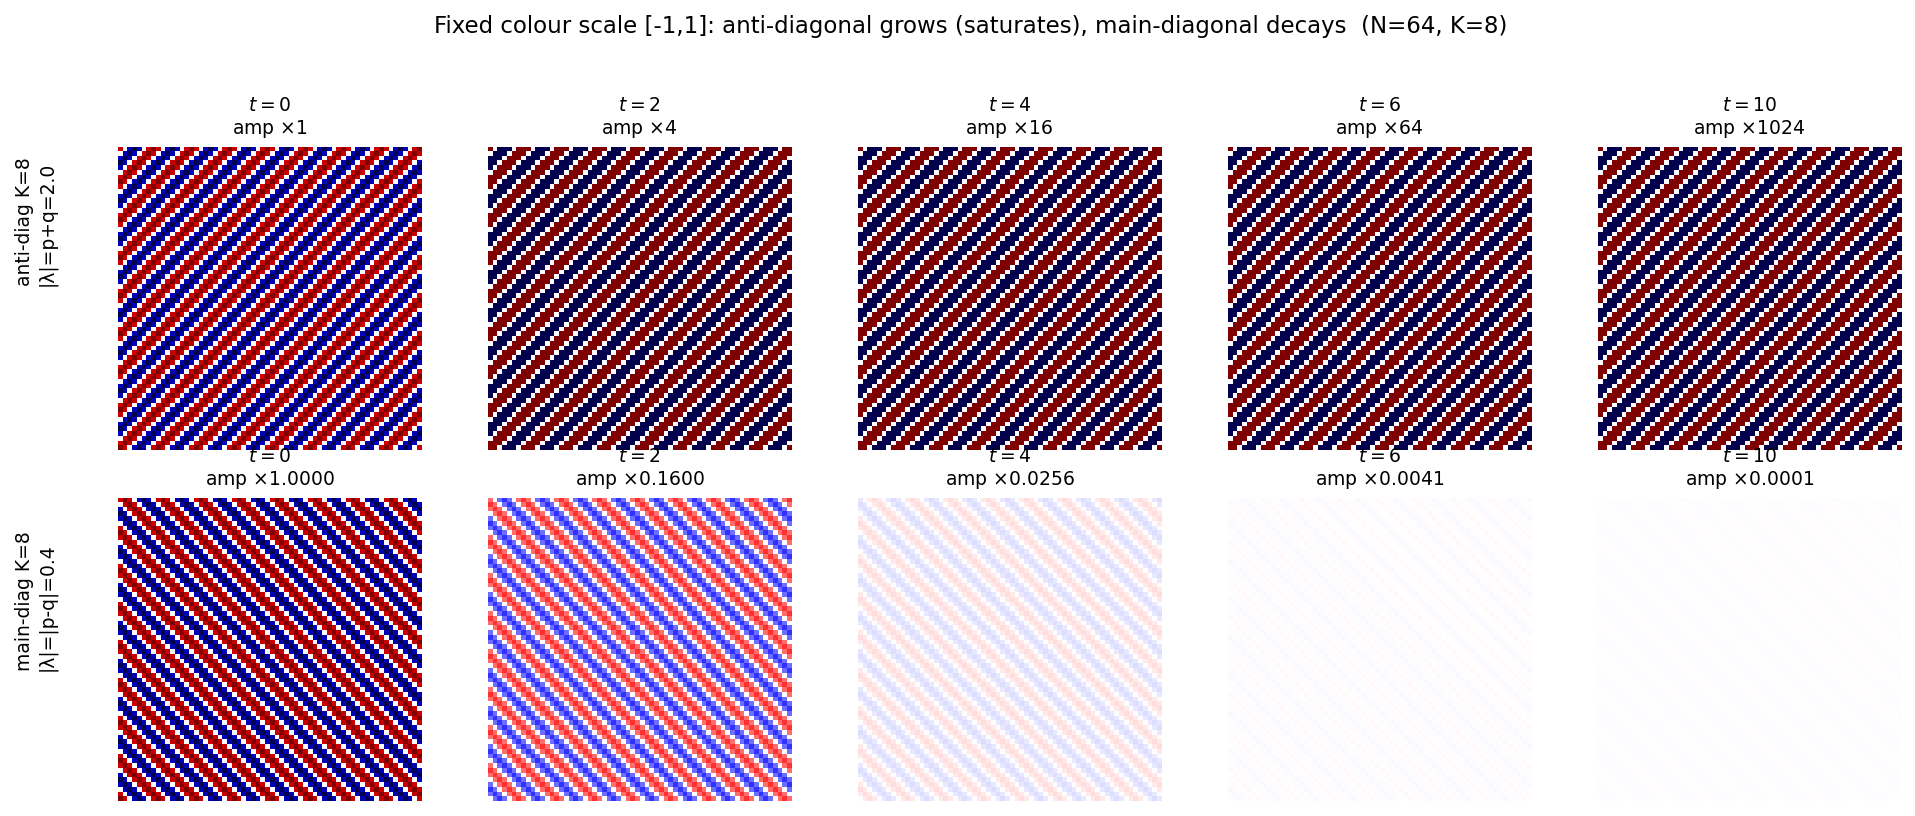
\includegraphics[width=\textwidth]{fig_stripes.png}
  \caption{Top row: anti-diagonal stripe $u=\cos(2\pi K(m-n)/N)$.
    Bottom row: main-diagonal stripe $u=\cos(2\pi K(m+n)/N)$.
    Each column is a time snapshot ($K=8$, amplitudes normalised).
    The anti-diagonal stripe stays a perfect stripe (only scaled);
    the main-diagonal stripe changes shape.}
\end{figure}

\noindent
Something striking:

\begin{enumerate}
  \item The \textbf{anti-diagonal stripe} $u_{m,n} = \cos(2\pi K(m-n)/N)$
    \emph{stays a clean stripe forever}.  It just scales: after $t$ steps
    its amplitude is $(p+q)^t = 2^t$ times the original, and its shape
    is unchanged.

  \item The \textbf{main-diagonal stripe} $u_{m,n} = \cos(2\pi K(m+n)/N)$
    \emph{does not stay the same shape}.  For large $K$ (short wavelength)
    it \emph{shrinks}; for small $K$ (long wavelength) it also grows, but
    at a different rate than $2^t$.
\end{enumerate}

\noindent
Check this quantitatively:

\begin{lstlisting}
for K in [1, 4, 8, 16, 32, 64]:
    u_a = wave(K, 'anti')
    u_m = wave(K, 'main')
    fa = simulate(u_a, T=1)
    fm = simulate(u_m, T=1)
    # amplitude ratio after one step
    ratio_a = np.max(np.abs(fa[1])) / np.max(np.abs(fa[0]))
    ratio_m = np.max(np.abs(fm[1])) / np.max(np.abs(fm[0]))
    print(f"K={K:3d}   anti-diag ratio = {ratio_a:.6f}   "
          f"main-diag ratio = {ratio_m:.6f}")
\end{lstlisting}

\noindent
You should see:
\begin{itemize}[nosep]
  \item \textbf{Anti-diagonal}: ratio $= p + q = 2.0$ for \emph{every} $K$.
  \item \textbf{Main diagonal}: ratio $= |p e^{2\pi i K/N \cdot 2} +
    q e^{-2\pi i K/N \cdot 2}|$, which equals
    $\sqrt{p^2 + q^2 + 2pq\cos(4\pi K/N)}$, ranging from $p+q=2.0$ (at
    $K=0$) down to $|p-q|=0.4$ (at $K=N/4$).
\end{itemize}

\medskip\noindent
The anti-diagonal direction is \emph{dispersion-free}: all wavelengths
travel at the same speed and grow at the same rate.  The main diagonal
direction is \emph{dispersive}: the growth rate depends on wavelength,
and short waves actually \emph{decay}.


% ================================================================
\section*{The Amplification Map}
% ================================================================

\noindent
Let us map out all modes at once.  Write a general plane wave as
\[
  u_{m,n} = e^{i(k_1 m + k_2 n)}, \qquad k_1, k_2 \in [0, 2\pi).
\]
The transfer operator acts on this wave as:
\begin{align*}
  (Tu)_{m,n}
  &= p\,e^{i(k_1(m+1)+k_2(n+1))} + q\,e^{i(k_1(m-1)+k_2(n-1))} \\
  &= \bigl(p\,e^{i(k_1+k_2)} + q\,e^{-i(k_1+k_2)}\bigr)\,e^{i(k_1 m+k_2 n)}.
\end{align*}
So every plane wave is an \textbf{eigenfunction} of $T$ with eigenvalue
\begin{equation}\label{eq:lam}
  \lambda(k_1,k_2) = p\,e^{i(k_1+k_2)} + q\,e^{-i(k_1+k_2)}.
\end{equation}
Note: $\lambda$ depends on $k_1$ and $k_2$ \emph{only through the
combination $k_1 + k_2$}.  This is the algebraic reason the main
diagonal direction $k_1 = k_2$ is special.

\medskip\noindent
The \emph{amplification factor} is
\[
  |\lambda(k_1,k_2)| = \sqrt{p^2 + q^2 + 2pq\cos\bigl(2(k_1+k_2)\bigr)}.
\]
Let us draw this as a heat map over the Brillouin zone
$[-\pi,\pi)^2$.

\begin{lstlisting}
k1 = np.linspace(-np.pi, np.pi, 512)
k2 = np.linspace(-np.pi, np.pi, 512)
K1, K2 = np.meshgrid(k1, k2, indexing='ij')

p, q = 1.2, 0.8
lam_abs = np.sqrt(p**2 + q**2 + 2*p*q*np.cos(2*(K1 + K2)))

fig, ax = plt.subplots(figsize=(7, 6))
cf = ax.contourf(k1, k2, lam_abs, levels=50, cmap='RdBu_r')
plt.colorbar(cf, ax=ax, label=r'$|\lambda(k_1, k_2)|$')
# Mark the stability boundary |lambda| = 1
ax.contour(k1, k2, lam_abs, levels=[1.0], colors='k', linewidths=2)

# Mark the two diagonal axes in the Brillouin zone
ax.axline((0, 0), slope= 1, color='lime',  lw=1.5, ls='--',
          label='main diagonal  $k_1 = k_2$')
ax.axline((0, 0), slope=-1, color='yellow', lw=1.5, ls='--',
          label='anti-diagonal  $k_1 = -k_2$')

ax.set(xlabel=r'$k_1$', ylabel=r'$k_2$',
       title=r'Amplification factor $|\lambda(k_1,k_2)|$ (black = stability boundary)')
ax.legend(loc='lower right')
plt.tight_layout(); plt.savefig("fig_amplification_map.png"); plt.show()
\end{lstlisting}

\begin{figure}[h!]
  \centering
  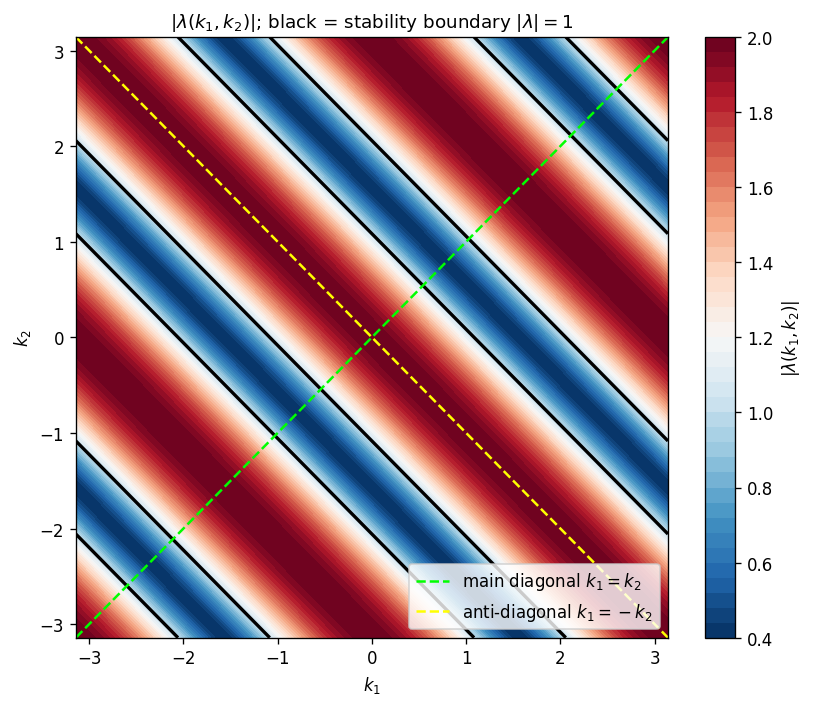
\includegraphics[width=0.82\textwidth]{fig_amplification_map.png}
  \caption{
    Amplification factor $|\lambda(k_1,k_2)|$ over the Brillouin zone
    $[-\pi,\pi)^2$.
    The black curve is the stability boundary $|\lambda|=1$;
    modes inside it grow ($|\lambda|>1$), modes outside decay ($|\lambda|<1$).
    The \textcolor{green}{green} dashed line is the main-diagonal axis
    $k_1=k_2$; the \textcolor{yellow}{yellow} dashed line is the
    anti-diagonal $k_1=-k_2$.
    \emph{(Run the code to generate this figure.)}
    Observe: the anti-diagonal axis lies \emph{entirely outside} the stability
    boundary (all modes grow at $|\lambda|=p+q=2$), while the main-diagonal
    axis \emph{crosses} the boundary (some modes grow, others decay).
  }
\end{figure}

\noindent
\textbf{What the map tells us.}
\begin{itemize}
  \item Every point on the anti-diagonal line $k_1 = -k_2$ satisfies
    $k_1 + k_2 = 0$, so $|\lambda| = \sqrt{p^2 + q^2 + 2pq} = p + q = 2.0$.
    All anti-diagonal modes are \emph{equally and maximally unstable}.

  \item The main-diagonal line $k_1 = k_2$ parametrises by $k_1+k_2 = 2k_1$,
    giving $|\lambda| = \sqrt{p^2+q^2+2pq\cos(4k_1)}$, which varies from
    $2.0$ (at $k_1=0$) to $|p-q| = 0.4$ (at $k_1 = \pi/2$).
    Modes near $k_1=k_2=\pi/2$ are \emph{strongly stable} --- they decay at
    $0.4^t$ per step.

  \item The \textbf{stability boundary} is the curve
    $\cos\bigl(2(k_1+k_2)\bigr) = -(p^2+q^2-1)/(2pq)$.
    For our parameters:
    $\cos(2(k_1+k_2)) = -(1.44 + 0.64 - 1)/(1.92) = -1.08/1.92 \approx -0.5625$.
    This gives $2(k_1+k_2) = \pm\arccos(-0.5625)$, so
    $k_1+k_2 = \pm 0.9742$ rad.
    The boundary consists of two \emph{diagonal lines} in the Brillouin zone.
\end{itemize}

\begin{lstlisting}
# Verify the stability boundary analytically
thresh = -(p**2 + q**2 - 1) / (2*p*q)
k_boundary = np.arccos(thresh) / 2
print(f"Stability boundary: k1+k2 = \pm{k_boundary:.4f} rad "
      f"(\approx \pm{np.degrees(k_boundary):.2f} deg)")
print(f"Check: |lambda| at boundary = "
      f"{np.sqrt(p**2+q**2+2*p*q*np.cos(2*k_boundary)):.6f}")
\end{lstlisting}


% ================================================================
\section*{A Calculation Anyone Can Verify}
% ================================================================

\noindent
The key computation behind all of this is a single line of algebra.
Take the anti-diagonal mode
\[
  u_{m,n} = e^{ik(m-n)}
  \quad\text{for any }k\in\mathbb{R}.
\]
Compute $(Tu)_{m,n}$:
\begin{align*}
  (Tu)_{m,n}
  &= p\,u_{m+1,n+1} + q\,u_{m-1,n-1} \\
  &= p\,e^{ik\bigl((m+1)-(n+1)\bigr)} + q\,e^{ik\bigl((m-1)-(n-1)\bigr)} \\
  &= p\,e^{ik(m-n)} + q\,e^{ik(m-n)} \\
  &= (p+q)\,e^{ik(m-n)} = (p+q)\,u_{m,n}.
\end{align*}
The north-east and south-west neighbours have \emph{exactly the same
value} as the centre, because both $(m+1)-(n+1)$ and $(m-1)-(n-1)$
equal $m-n$.  Hence $T$ acts as scalar multiplication $(p+q) = 2$ on
\emph{every} anti-diagonal mode regardless of $k$.

\medskip\noindent
Contrast with the main-diagonal mode $v_{m,n} = e^{ik(m+n)}$:
\begin{align*}
  (Tv)_{m,n}
  &= p\,e^{ik(m+1+n+1)} + q\,e^{ik(m-1+n-1)} \\
  &= p\,e^{2ik}\,e^{ik(m+n)} + q\,e^{-2ik}\,e^{ik(m+n)} \\
  &= \bigl(p\,e^{2ik}+q\,e^{-2ik}\bigr)\,v_{m,n}.
\end{align*}
The eigenvalue $\lambda_k = p e^{2ik} + q e^{-2ik}$ has magnitude
$\sqrt{p^2+q^2+2pq\cos 4k}$, which \emph{depends on $k$}.  At
$k = \pi/4$ the two terms interfere destructively and
$|\lambda_{\pi/4}| = |p-q| = 0.4 < 1$.

\medskip\noindent
\textbf{What this means geometrically.}
The anti-diagonal mode $e^{ik(m-n)}$ is \emph{constant along each
main-diagonal line} $\{(m+j,n+j):j\in\mathbb{Z}\}$.  Since the
operator $T$ samples the two main-diagonal neighbours, it ``sees''
the same value everywhere along its coupling axis; the computation
becomes trivial.  The main-diagonal mode, by contrast, \emph{oscillates}
along the coupling axis, and the oscillations interfere.

\begin{lstlisting}
# Numerical verification of the eigenvalue formula
errors = []
for K in np.linspace(0, np.pi, 100):
    u = np.cos(K * (m_idx - n_idx))     # anti-diagonal mode (real part)
    v = step(u)                          # apply T
    # T should multiply by (p+q); check the ratio pointwise
    ratio = v / (u + 1e-14)             # avoid division by zero
    errors.append(np.std(ratio[np.abs(u) > 0.5]))  # std of ratio on large cells

print(f"Anti-diagonal: max std of ratio over all k = {max(errors):.2e}")
# Should be ~machine precision

errors_main = []
for K in np.linspace(0, np.pi, 100):
    u = np.cos(K * (m_idx + n_idx))     # main-diagonal mode
    v = step(u)
    lam_pred = p * np.exp(2j*K) + q * np.exp(-2j*K)
    ratio = v / (u + 1e-14)
    errors_main.append(np.std(ratio[np.abs(u) > 0.5]))

print(f"Main-diagonal:  max std of ratio over all k = {max(errors_main):.2e}")
# Should also be ~machine precision, just to confirm the formula
\end{lstlisting}


% ================================================================
\section*{Decomposing Any Initial Condition}
% ================================================================

\noindent
Every function on $\mathbb{Z}^2$ decomposes into plane waves via the
\textbf{2D discrete Fourier transform}:
\[
  u_{m,n} = \frac{1}{N^2} \sum_{k_1,k_2} \hat{u}_{k_1,k_2}\,
            e^{2\pi i(k_1 m + k_2 n)/N}.
\]
Since $T$ multiplies each mode $e^{i(k_1 m + k_2 n)}$ by
$\lambda(k_1,k_2)$, after $t$ steps:
\[
  (T^t u)_{m,n} = \frac{1}{N^2} \sum_{k_1,k_2} \hat{u}_{k_1,k_2}\,
  \lambda(k_1,k_2)^t\,e^{2\pi i(k_1 m + k_2 n)/N}.
\]
Modes with $|\lambda| > 1$ amplify; modes with $|\lambda| < 1$ die.
In the long run, only the largest-$|\lambda|$ modes survive.

\medskip\noindent
\textbf{Verify with the FFT.}

\begin{lstlisting}
def predict_fft(u0, t, p=1.2, q=0.8):
    """Predict T^t u0 using the exact eigenvalue formula."""
    Uhat = np.fft.fft2(u0)                         # Fourier transform
    N = u0.shape[0]
    k1 = 2 * np.pi * np.fft.fftfreq(N)            # frequencies in [-pi, pi)
    K1, K2 = np.meshgrid(k1, k1, indexing='ij')
    lam = p * np.exp(1j*(K1+K2)) + q * np.exp(-1j*(K1+K2))
    Uhat_t = Uhat * (lam ** t)                     # multiply by eigenvalue^t
    return np.real(np.fft.ifft2(Uhat_t))           # inverse transform

# Random initial condition
np.random.seed(42)
u0 = np.random.randn(N, N) * 0.01   # small random noise on 256x256 grid

T_test = 15
u_sim  = simulate(u0, T=T_test)[-1]
u_pred = predict_fft(u0, T_test)

print(f"Max absolute error between simulation and FFT prediction: "
      f"{np.max(np.abs(u_sim - u_pred)):.2e}")
# Should be < 1e-10: perfect agreement
\end{lstlisting}

\noindent
The prediction is exact (up to floating-point rounding).  We can
predict the state after any number of steps in $O(N^2 \log N)$ time
using the FFT, rather than iterating the rule $t$ times.


% ================================================================
\section*{The Glider Revisited}
% ================================================================

\noindent
A GoL glider is a coherent structure that moves diagonally.
In our linear model, coherent diagonal-travelling patterns are
precisely the \emph{anti-diagonal modes} $e^{ik(m-n)}$: they travel
in the $m-n = \text{const}$ direction (anti-diagonal, i.e.,
$(+1,-1)$ and $(-1,+1)$) and grow uniformly without dispersion.

\medskip\noindent
Both GoL and our rule are \emph{neighbour-sum} rules.
GoL counts all eight Moore neighbours and applies a threshold;
our rule takes a weighted sum of the two diagonal neighbours without a
threshold.
Ours is, in a loose sense, the \emph{linear, diagonal-only
simplification} of GoL.

\medskip\noindent
In our model, anti-diagonal modes are eigenvectors with eigenvalue
$p+q$ for \emph{every} wavelength: diagonal neighbours of an
anti-diagonal wave always carry the same phase as the centre, so
the neighbour sum adds up the same way regardless of $k$.
The GoL glider exploits the same diagonal geometry: the specific
five-cell pattern arranges its diagonal neighbours to reproduce
exactly the right counts step after step.
In both cases it is the diagonal neighbour structure that makes
coherent diagonal motion possible.

\medskip\noindent
The full story for GoL requires nonlinear analysis.
But eigenvalue thinking --- understanding which directions the rule
treats uniformly --- is the right first step.

\begin{lstlisting}
# Illustrate: anti-diagonal wave travels as a coherent wave
# Main-diagonal wave at the same frequency disperses
K_test = 16
u_anti_init = wave(K_test, 'anti')
u_main_init = wave(K_test, 'main')

# After 30 steps: anti-diagonal should look like a scaled/shifted original;
# main-diagonal should look different (dispersed for large K)
u_anti_30 = predict_fft(u_anti_init, 30)
u_main_30 = predict_fft(u_main_init, 30)

# Normalise for visual comparison
def norm(u): return u / (np.max(np.abs(u)) + 1e-14)

fig, axes = plt.subplots(2, 2, figsize=(12, 10))
axes[0,0].imshow(norm(u_anti_init), cmap='seismic', vmin=-1, vmax=1,
                 origin='lower'); axes[0,0].set_title('Anti-diag, t=0')
axes[0,1].imshow(norm(u_anti_30),  cmap='seismic', vmin=-1, vmax=1,
                 origin='lower'); axes[0,1].set_title('Anti-diag, t=30')
axes[1,0].imshow(norm(u_main_init), cmap='seismic', vmin=-1, vmax=1,
                 origin='lower'); axes[1,0].set_title('Main-diag, t=0')
axes[1,1].imshow(norm(u_main_30),  cmap='seismic', vmin=-1, vmax=1,
                 origin='lower'); axes[1,1].set_title('Main-diag, t=30  (dispersed?)')
plt.suptitle(f"Coherence of diagonal waves after 30 steps  (K={K_test})")
plt.tight_layout(); plt.savefig("fig_diagonal_compare.png"); plt.show()
\end{lstlisting}

\begin{figure}[h!]
  \centering
  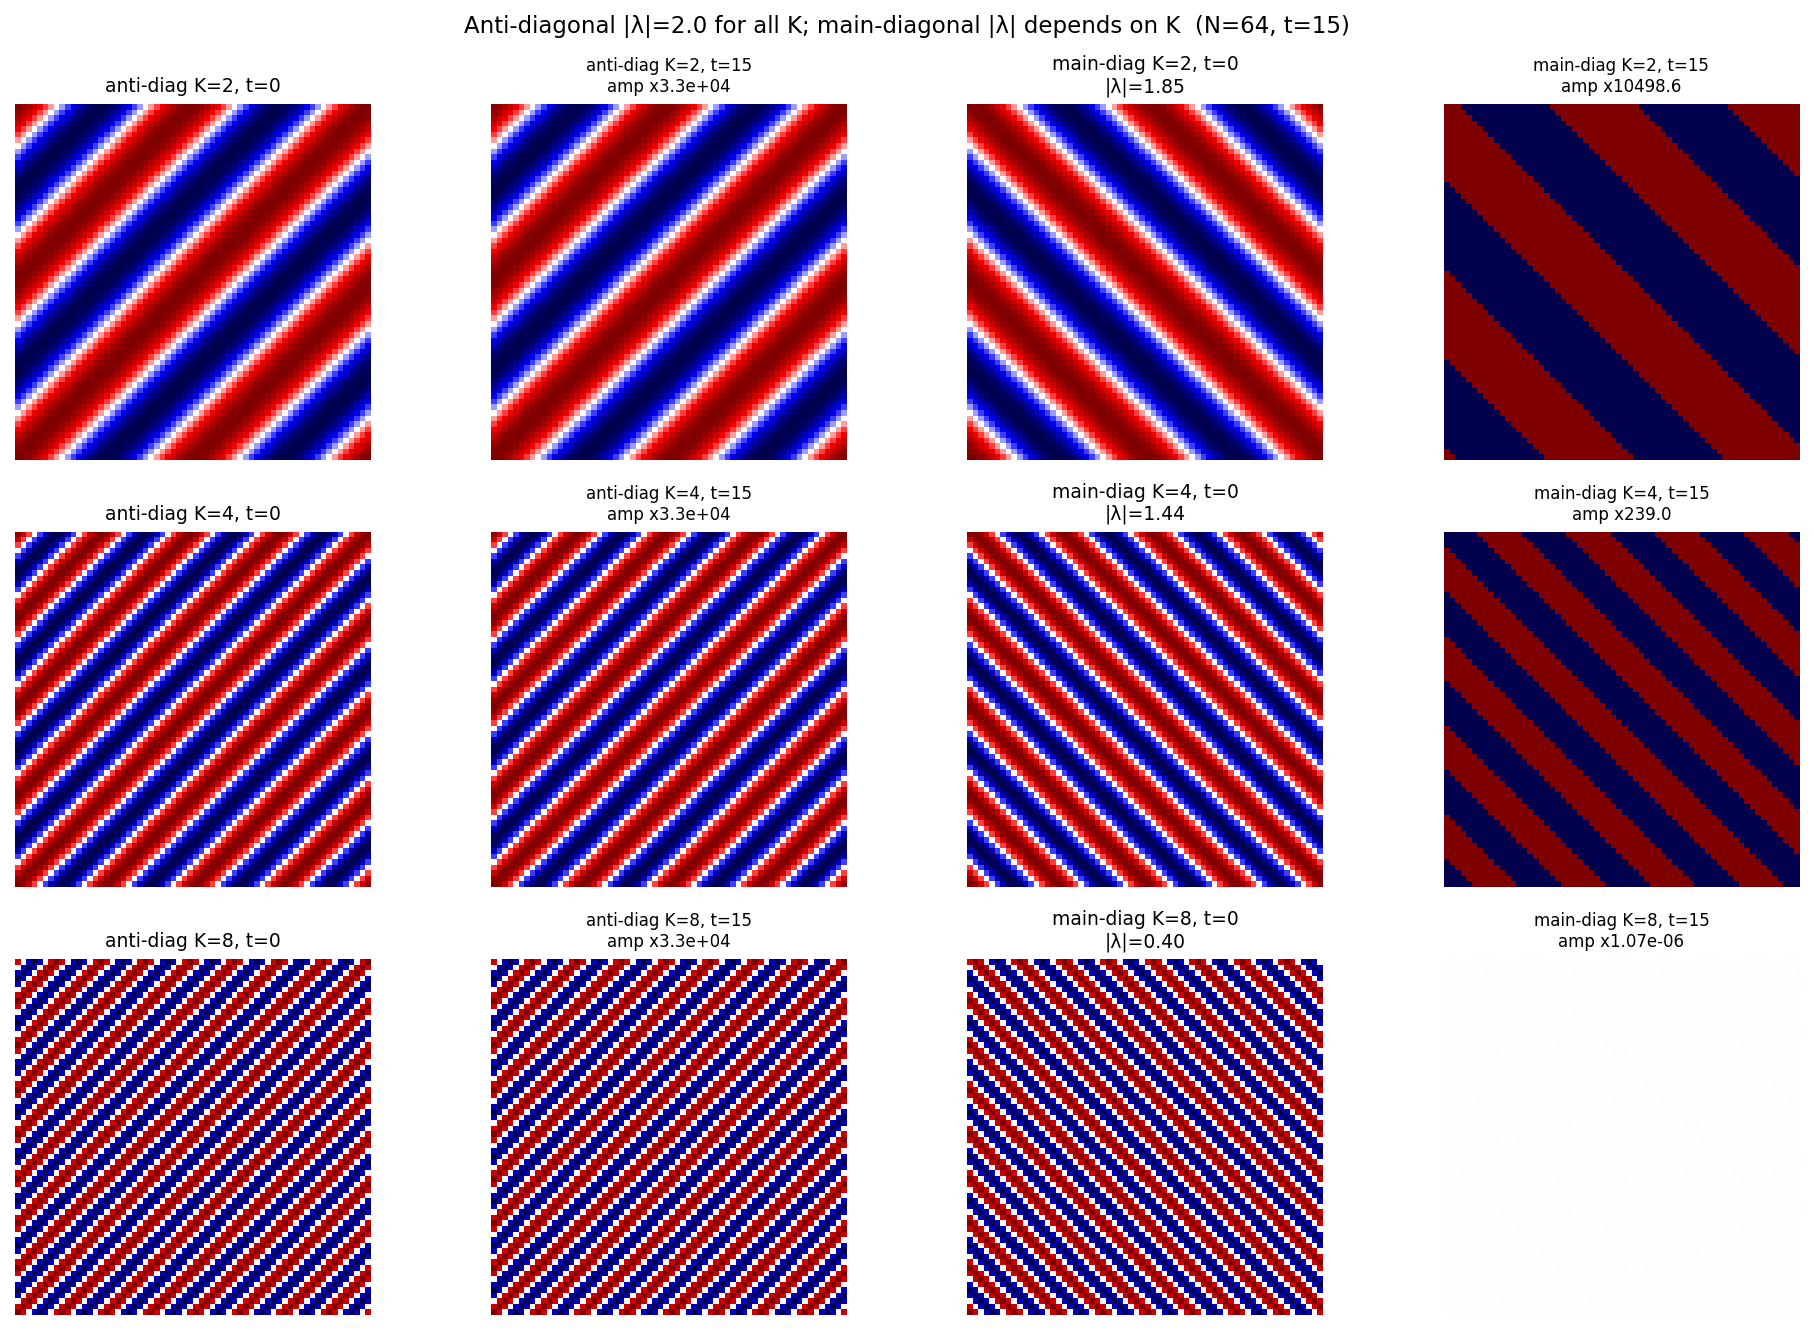
\includegraphics[width=\textwidth]{fig_diagonal_compare.png}
  \caption{Each row shows a wavenumber $K\in\{4,16,48\}$ at $t=0$ and $t=30$
    (amplitudes normalised).
    Anti-diagonal waves (left two columns) remain perfect stripes at all $K$.
    Main-diagonal waves (right two columns) stay coherent at long wavelength
    ($K=4$) but dissolve at short wavelength ($K=48$): dispersion in action.}
\end{figure}

\noindent
Try different values of $K$ and observe when the main-diagonal wave
disperses (short wavelength, $K$ near $N/4$) vs.\ when it stays roughly
coherent (long wavelength, $K$ small).


% ================================================================
\section*{Things We Can and Cannot Do}
% ================================================================

\renewcommand{\arraystretch}{1.5}
\begin{center}
\begin{tabular}{@{}p{0.055\textwidth}p{0.43\textwidth}p{0.43\textwidth}@{}}
\toprule
& \textbf{Question} & \textbf{Status} \\
\midrule
\checkmark
& Does an anti-diagonal stripe grow or decay?
& \emph{Grows at rate $p+q = 2$ per step} --- proved by direct computation. \\

\checkmark
& Does a main-diagonal short-wave mode grow or decay?
& \emph{Decays at rate $|p-q| = 0.4$} --- eigenvalue formula. \\

\checkmark
& Predict $T^t u_0$ exactly for any $u_0$?
& \emph{Yes, via FFT}: $O(N^2 \log N)$, verified numerically. \\

\checkmark
& What is the stability boundary in frequency space?
& \emph{Two diagonal lines} $k_1+k_2 = \pm\arccos(-(p^2+q^2-1)/2pq)$. \\
\midrule

$\times$
& Why does $|\lambda|$ depend only on $k_1+k_2$ and nothing else?
& \emph{Unknown yet.}  The rule~\eqref{eq:T} is translation-invariant in the
  anti-diagonal direction; this is equivalent to saying $T$ commutes with
  a certain operator.  The general framework is spectral theory of
  translation-invariant operators on $\ell^2(\mathbb{Z}^2)$. \\

$\times$
& Add nearest-neighbour coupling as well:
  $u_{m,n}^{t+1} = p u_{m+1,n+1}^t + q u_{m-1,n-1}^t
               + r(u_{m+1,n}^t + u_{m-1,n}^t + u_{m,n+1}^t + u_{m,n-1}^t)$.
  How does the stability map change?
& \emph{Unknown yet.}  With $r\ne 0$ the rule is no longer diagonal-only;
  the formula for $\lambda(k_1,k_2)$ changes and the two diagonal directions
  are no longer distinguished.  (Try it --- the anti-diagonal modes no longer
  all share the same $|\lambda|$.) \\

$\times$
& Same rule but on a \emph{finite strip} with reflecting boundaries?
& \emph{Unknown yet.}  Fourier modes no longer fit.  We need eigenvectors of
  a \emph{matrix} (not a convolution operator), found by eigenvalue decomposition. \\

$\times$
& Non-uniform parameters: $p_{m,n}$ and $q_{m,n}$ vary across the grid
  (like a terrain with varying diffusion, or GoL with varying rules).
& \emph{Unknown yet.}  Translation invariance breaks; the entire Fourier
  approach fails.  Need eigenvectors of a large (possibly sparse) matrix. \\

$\times$
& Can we \emph{design} $p$ and $q$ to make a target mode
  exactly neutral ($|\lambda|=1$)?
& \emph{Unknown yet.}  Requires solving an inverse problem in terms of
  eigenvalues. \\

$\times$
& GoL is nonlinear.  Does it also have something analogous to
  ``diagonal eigenmodes''?
& \emph{Unknown yet.}  Stability near fixed points of GoL is governed by the
  \emph{Jacobian matrix} (the linearisation), whose spectrum we would need. \\

\bottomrule
\end{tabular}
\end{center}


% ================================================================
\section*{The Road Ahead}
% ================================================================

\noindent
Every ``unknown yet'' row in the table above points to something the
course will teach you to handle.

\medskip
\begin{enumerate}[leftmargin=2em, itemsep=4pt]
  \item \textbf{Vector spaces and linear maps.}
    The space $\ell^2(\mathbb{Z}^2) = \{u:\mathbb{Z}^2\to\mathbb{R} :
    \sum_{m,n}u_{m,n}^2 < \infty\}$ is an infinite-dimensional
    \emph{vector space}.  The transfer operator $T$ is a \emph{linear map}
    on it.  The same concepts (kernel, image, rank, dimension) apply,
    but now in infinite dimensions.

  \item \textbf{Eigenvalues and eigenvectors.}
    The plane waves $e^{i(k_1 m + k_2 n)}$ are
    \emph{eigenvectors} of $T$, with eigenvalues $\lambda(k_1,k_2)$.
    For the rule~\eqref{eq:T}, the eigenvalue depends only on $k_1+k_2$
    --- a symmetry we will explain rigorously.

  \item \textbf{Spectral decomposition / diagonalisation.}
    The identity $T^t u_0 = \mathcal{F}^{-1}[\lambda^t \cdot \hat u_0]$
    is a \emph{diagonalisation}: we change to the ``eigenbasis''
    (Fourier modes), multiply each component by $\lambda^t$, and change
    back.  For finite matrices this becomes $T = V \Lambda V^{-1}$,
    $T^t = V \Lambda^t V^{-1}$.

  \item \textbf{Commuting operators and simultaneous diagonalisation.}
    The reason ALL anti-diagonal modes share $|\lambda|=p+q$ is that
    $T$ \emph{commutes} with the anti-diagonal translation operator
    $S_{(1,-1)}$.  Two commuting diagonalisable operators can always be
    simultaneously diagonalised.  This is why the
    anti-diagonal Fourier basis diagonalises both.

  \item \textbf{Operator theory and the Spectral Theorem.}
    What happens when the operator is not convolution, or when we are
    on a finite domain?  The Spectral Theorem (for symmetric/Hermitian
    operators) guarantees orthogonal eigenbases.  The
    Singular Value Decomposition handles the non-symmetric case.

  \item \textbf{Stability and the spectrum.}
    A linear dynamical system is \emph{stable} iff all eigenvalues
    satisfy $|\lambda|\le 1$.  For our rule the stability boundary is a
    curve in frequency space; understanding it requires knowing the full
    spectrum.  This is directly relevant to numerical PDE solvers,
    control theory, and the long-run behaviour of GoL linearisations.
\end{enumerate}

\bigskip\noindent
\textbf{One exercise to carry with you.}

Add a small axis-aligned coupling:
\[
  u_{m,n}^{t+1} = p\,u_{m+1,n+1}^t + q\,u_{m-1,n-1}^t
    + r\bigl(u_{m+1,n}^t + u_{m-1,n}^t + u_{m,n+1}^t + u_{m,n-1}^t\bigr)
\]
with $r = 0.05$.

\begin{lstlisting}
def step_full(u, p=1.2, q=0.8, r=0.05):
    diag  = p * np.roll(np.roll(u,-1,0),-1,1) + q * np.roll(np.roll(u,+1,0),+1,1)
    axis  = r * (np.roll(u,-1,0) + np.roll(u,+1,0)
               + np.roll(u,-1,1) + np.roll(u,+1,1))
    return diag + axis

# Re-run all experiments above with step_full instead of step.
# Does the anti-diagonal still have |lambda| = 2 for all k?
# Does the stability map change shape?
\end{lstlisting}

\begin{figure}[h!]
  \centering
  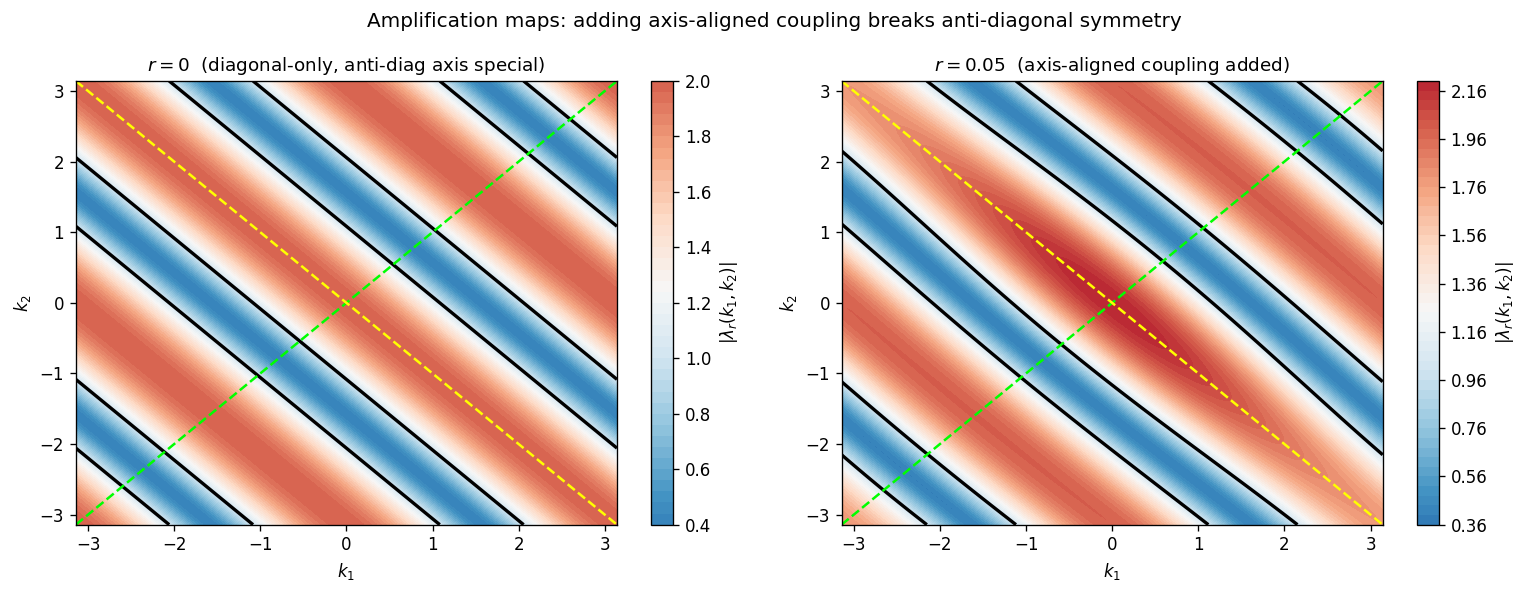
\includegraphics[width=\textwidth]{fig_perturbation.png}
  \caption{Amplification maps for $r=0$ (left) and $r=0.05$ (right).
    At $r=0$ the map depends only on $k_1+k_2$: the anti-diagonal axis
    (yellow dashes) has constant $|\lambda|=2$ everywhere.
    At $r=0.05$ that symmetry is broken: the anti-diagonal is no longer special.}
\end{figure}

\noindent
The new eigenvalue is
$\lambda_r(k_1,k_2) = pe^{i(k_1+k_2)} + qe^{-i(k_1+k_2)}
  + 2r(\cos k_1 + \cos k_2)$.
For $r \ne 0$, this no longer depends only on $k_1+k_2$; the
anti-diagonal is no longer special.  With $r = 0.05$, compute the
new stability map and find: does any diagonal direction remain special?
Can you explain geometrically why the perturbation breaks the
anti-diagonal symmetry?

\vspace{2em}
\begin{center}
\hrulefill\hspace{0.2cm}%
\pgfornament[width=0.9cm,ydelta=-3pt,symmetry=v]{79}\hspace{0.15cm}%
{\large\floweroneleft\floweroneright}%
\hspace{0.15cm}\pgfornament[width=0.9cm,ydelta=-3pt]{79}%
\hspace{0.2cm}\hrulefill
\end{center}

\end{document}
